\section{Strimzi system tests}
\label{02:sec:strimzisystemtests}

This section describes the basics of the Strimzi system tests.
We start with a short description of any way we test the Strimzi product.
Then in the section \ref{02d-strimzi-architecture} we explain the architecture of the core parts in Strimzi system tests and describe the individual supporting components. Finally, in the\ref{02d-strimzi-algorithm} section, we describe the algorithms that are available for overall resource management.

It all starts with a typical regression, where we start with unit tests, integration tests, and system tests. Of course, the most time-consuming is system tests, which in our case take about 40 hours. The testing phases are dependent on each other in the order in which they are executed. For instance, if unit tests fail, integration tests will not run at all. The same is true for integration and system tests. System tests run on multiple infrastructures such as Openstack, Microsoft Azure or Amazon Web Services. On each of these infrastructures, there are certain limitations for the set of tests. Since these are Kubernetes system tests, it is essential to realize that the total load on the resource is enormous. At the same time, the preparation of resources and their cleaning is time-consuming. Therefore, our system tests have two essential parts. The first is resource classes that provide the user interface for creating, retrieving, deleting, and updating these resources. Moreover, we have three stacks that take care of the total lifecycle test. These stacks are responsible for storing all resources based on the test case. Furthermore, the deletion of these resources is transparent for the user as well as if it is a resource created in \emph{@BeforeAll}\footnote{\textbf{@BeforeAll } \---\ is JUnit5 annotation, where one specify what must be executed before all tests in the test suite.} annotation. The second fundamental part is auxiliary classes such as Utils\footnote{\textbf{Utils} \---\ type of class that consists of static methods, which in general dynamically waiting for a specific event. For instance, waiting for Rolling Update, if one change Kafka configuration}, Apache Kafka clients for external communication, Kubernetes client offering an API for communication with the Kubernetes cluster and finally classes such as Constants and Environment.

\subsection{Architecture}
\label{02d-strimzi-architecture}

Each resource has his own creation method which is not good practice. For instance Kafka resources has default instance predefined like this:

\begin{figure}[!ht]
    \centering
    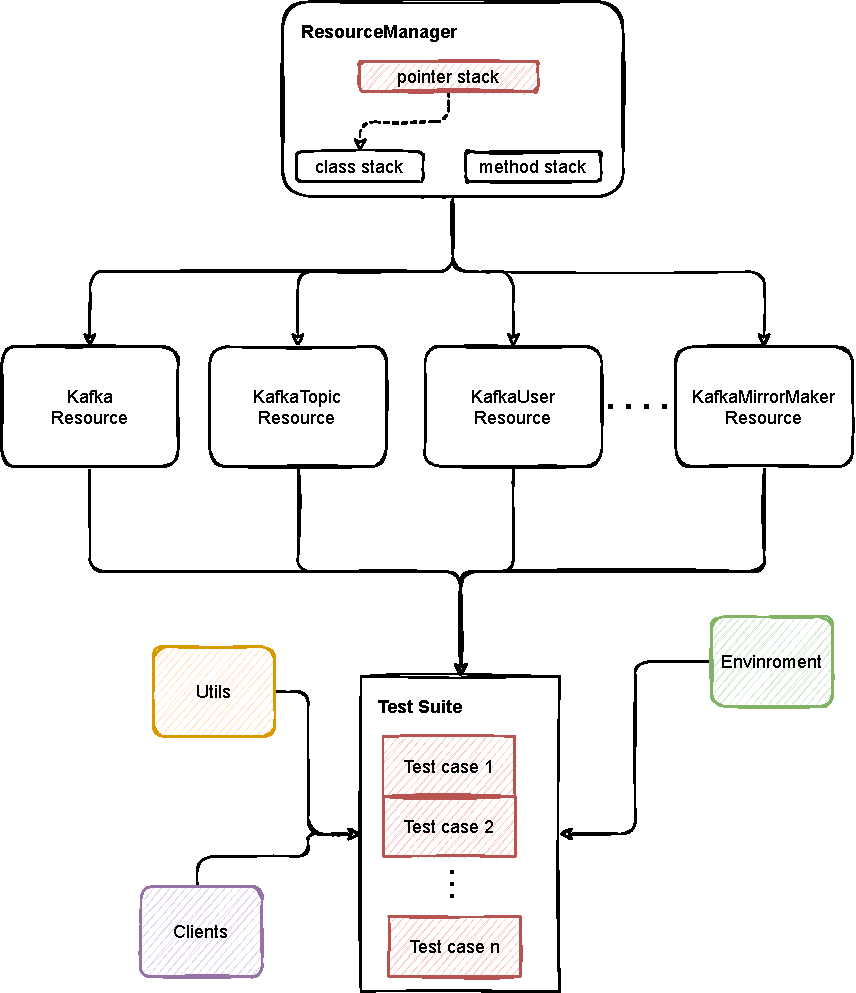
\includegraphics[scale=0.70]{obrazky-figures/02-preliminaries/04-strimzi-system-tests/01-architecture-overall.pdf}
    \caption{Strimzi Kafka architecture}
    \label{04:fig:strimzi}
\end{figure}

\begin{itemize}[itemsep=1mm, parsep=0pt]
    \item also add here some diagram, which will show communication between components
    \item another diagram how it is called (relation between templates, user, creation and deletion methods), resource manager and so on...
\end{itemize}

\begin{verbatim}
private static KafkaBuilder defaultKafka(
            Kafka kafka,
            String name,
            int kafkaReplicas,
            int zookeeperReplicas) {
    return new KafkaBuilder(kafka)
        .withNewMetadata()
            .withName(name)
            .withNamespace(ResourceManager.kubeClient().getNamespace())
        .endMetadata()
        .editSpec()
            .editKafka()
                .withVersion(Environment.ST_KAFKA_VERSION)
                .withReplicas(kafkaReplicas)
            .endKafka()
            .editZookeeper()
            .endZookeeper()
            .editEntityOperator()
            .endEntityOperator()
\end{verbatim}

\begin{algorithm}[H]
    \label{01:alg:dsds}
    \caption{Sequential algorithm for creation all resources inside \emph{Resource manager}}

    \begin{algorithmic}[1]
        \State start\_here
    \end{algorithmic}
\end{algorithm}


\begin{algorithm}[H]
    \label{01:alg:dsdsd+}
    \caption{Sequential algorithm for deletion all resources inside \emph{Resource manager}}

    \begin{algorithmic}[1]
        \State start\_here
    \end{algorithmic}
\end{algorithm}


\subsection*{Implementation}